

??? TO DO

\begin{figure}[!htb]
	\centering
	\resizebox{0.5\columnwidth}{!}{
	\begin{tikzpicture}[genericStyle]
  % Define the lengths for horizontal and vertical skips
  \def\vSkip{1}
  \def\hSkip{1}
  \def\vExtra{0.25}
  \def\myRad{0.75}
  \def\myRadH{0.3}
  \def\myCornerIn{5}
  \def\myCornerOut{5}
  \def\vClip{2}
  \def\vLead{0.3}

  % Cylinder 1
  \begin{scope}
    \draw[draw=none, name path=Hleft] (-\myRad,0) {[rounded corners=\myCornerIn] -- ++(0,\vExtra+\vSkip)} {[rounded corners=\myCornerOut]-- ++(\hSkip,\vSkip) -- ++(0,\vSkip+\vLead)};

    \draw[draw=none, name path=Hright] (\myRad,0) {[rounded corners=\myCornerOut] -- ++(0,\vSkip)} {[rounded corners=\myCornerIn]-- ++(\hSkip,\vSkip) -- ++(0,\vExtra+\vSkip+\vLead)};

    \tikzfillbetween[of=Hleft and Hright]{topologyFillColor};
  \end{scope}

  \begin{scope}
    \draw[darkgray, name path=Hleft] (-\myRad,0) {[rounded corners=\myCornerIn] -- ++(0,\vExtra+\vSkip)} {[rounded corners=\myCornerOut]-- ++(\hSkip,\vSkip) -- ++(0,\vSkip+\vLead)};

    \draw[darkgray, name path=Hright] (\myRad,0) {[rounded corners=\myCornerOut] -- ++(0,\vSkip)} {[rounded corners=\myCornerIn]-- ++(\hSkip,\vSkip) -- ++(0,\vExtra+\vSkip+\vLead)};
  \end{scope}

  % Cylinder 2

  \begin{scope}
    \draw[draw=none, name path=Dleft] (\myRad,0) {[rounded corners=\myCornerIn] -- ++(0,\vExtra+\vSkip)} {[rounded corners=\myCornerOut]-- ++(-\hSkip,\vSkip) -- ++(0,\vSkip)};

    \draw[draw=none, name path=Dright] (-\myRad,0) {[rounded corners=\myCornerOut] -- ++(0,\vSkip)} {[rounded corners=\myCornerIn]-- ++(-\hSkip,\vSkip) -- ++(0,\vSkip+\vExtra)};

    \tikzfillbetween[of=Dleft and Dright]{topologyFillColor};
  \end{scope}

  \begin{scope}
    \clip (-\hSkip,1.75) rectangle (\hSkip,3.5);

    \draw[darkgray] (\myRad,0) {[rounded corners=\myCornerIn] -- ++(0,\vExtra+\vSkip)} {[rounded corners=\myCornerOut]-- ++(-\hSkip,\vSkip) -- ++(0,\vSkip)};
  \end{scope}

  \draw[darkgray] (-\myRad,0) {[rounded corners=\myCornerOut] -- ++(0,\vSkip)} {[rounded corners=\myCornerIn]-- ++(-\hSkip,\vSkip) -- ++(0,\vSkip+\vExtra)};

  \begin{scope}
    \draw[darkgray, name path=Hright] (\myRad,0) {[rounded corners=\myCornerOut] -- ++(0,\vSkip)} {[rounded corners=\myCornerIn]-- ++(\hSkip,\vSkip) -- ++(0,\vExtra+\vSkip)};
  \end{scope}

  % Ellipses
  \draw[gray, dashed, fill=setHDFillColor, myShadow] (-\myRad,0) arc [start angle=0, end angle=180, x radius=-\myRad, y radius =\myRadH];
  \draw[darkgray, fill=setHDFillColor, myShadow] (-\myRad,0) arc [start angle=0, end angle=-180, x radius=-\myRad, y radius =\myRadH];

  \draw[darkgray, fill=setDFillColor] (\hSkip-\myRad,3*\vSkip+\vExtra+\vLead) arc [start angle=0, end angle=180, x radius=-\myRad, y radius =\myRadH];
  \draw[darkgray, fill=setDFillColor] (\hSkip-\myRad,3*\vSkip+\vExtra+\vLead) arc [start angle=0, end angle=-180, x radius=-\myRad, y radius =\myRadH];

  \draw[darkgray, fill=setHFillColor] (-\hSkip-\myRad,3*\vSkip+\vExtra) arc [start angle=0, end angle=180, x radius=-\myRad, y radius =\myRadH];
  \draw[darkgray, fill=setHFillColor] (-\hSkip-\myRad,3*\vSkip+\vExtra) arc [start angle=0, end angle=-180, x radius=-\myRad, y radius =\myRadH];

  % Latex
  \node[draw=none] at (0,0) {$\mathcal{N}$};
  \node[draw=none] at (-\hSkip,3*\vSkip+\vExtra) {$\mathcal{N}_H$};
  \node[draw=none] at (\hSkip,3*\vSkip+\vExtra+\vLead) {$\mathcal{N}_D$};

\end{tikzpicture}
	}
	\caption{\textbf{Bifurcation in network trust.} When the network \mbox{$\mathcal{N}=\mathcal{N}_H\cup\mathcal{N}_D$} supporting a blockchain segregates into two non-interacting networks, $\mathcal{N}_H$ and $\mathcal{N}_D$, a fork is created, forming two unique, legitimate blockchains, one associated with each network.} \label{fig:forking}
\end{figure}

\begin{figure}[!htb]
	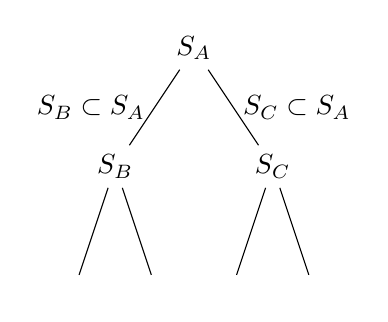
\begin{tikzpicture}
		[level distance=15mm,level/.style={sibling distance=20mm/#1}]
		\node {$S_A$}
		child {node {$S_B$}
				child {node {}}
				child {node {}}
				edge from parent node[left,draw=none] {$S_B\subset S_A$}
			}
		child {node {$S_C$}
				child {node {}}
				child {node {}}
				edge from parent node[right,draw=none] {$S_C\subset S_A$}
			};
	\end{tikzpicture}
	\caption{Trust hierarchies represented as subset-trees define retreat strategies.} \label{fig:subset_tree}
\end{figure}

Fig.~\ref{fig:subset_tree}

`Rebasing' network upon strategic retreat.

Retreat strategy in trust hierarchy where root is level $i=0$. Levels represent set containment, $s_{i+1}\subset s_i$. Retreat to smallest i (i.e largest trusted subset). Assume that $r_{i+1}<r_i$. Inequality could work in either direction??
